\documentclass{article} 
\usepackage[left=0.75in,top=0.6in,right=0.75in,bottom=0.6in]{geometry} % Document margins
\usepackage{tabularx}
\usepackage{fancyvrb}
\usepackage{graphicx}
\usepackage{multicol,caption}
\usepackage{fancyhdr}
\usepackage{lipsum}
\usepackage{mathtools}
\usepackage{float}
\usepackage{textcomp}

%Header Stuff
\newenvironment{Figure}
  {\par\medskip\noindent\ignorespaces\minipage{\linewidth}}
  {\endminipage\par\medskip}

\usepackage{fancyhdr}
\pagestyle{fancy}
\fancyhf{}
\renewcommand{\headrulewidth}{0pt}
\fancyhead[R]{\thepage}


\begin{document}

%----------------------------------------------------------------------------------------
%		 TITLE 
%----------------------------------------------------------------------------------------
\begin{center}

\vspace* {15 pt}
\Huge{\bf Performing image processing and display using DE2-115 FPGA}\\
\vspace {20 pt}
\large{Howard Edwards, Michael Micros, Jonathon  Rigney, Megan Rowland \\}

\end{center}

\vspace{15 pt}




\begin{multicols*}{2}

%----------------------------------------------------------------------------------------
%		ABSTRACT
%----------------------------------------------------------------------------------------
{\bf  \textit {Abstract(Jonathon Rigney)} ---}
\par 
This report is a part of a series of papers aimed at designing and implementing a system to perform real time video processing using a Field Programmable Gate Array(FPGA). This paper focuses on the image processing functions of an FPGA loaded with an Altera Media Computer along with the communication between the FPGA, a user controlled interface(GUI), and a separate display monitor. The user sends an image from a QT GUI to the FPGA to process through a serial connection, after the image is processed it is displayed via VGA onto the second monitor. This processing will convert the image from RGB to Grayscale. 



{\bf  \textit {Index Terms} --- FPGA, Signal Processing}



%----------------------------------------------------------------------------------------
%		INTRODUCTION
%----------------------------------------------------------------------------------------

\begin{center}
\large{I. Introduction(Howard Edwards)}
\end{center}
\par   The main focus of this report is to document a stage in the development of a project. The project is the creation of an integrated system that performs the processing of real-time video through a graphical user-interface, GUI, on a computer and the use of field-programmable gate arrays, FPGAs. This stage of the project displays image data on an external monitor.

     The previous stages of the project were documented in reports by Edwards, Micros et al[1][2][3][4]. Working from the previous stages of the project, the GUI was modified, and the media computer and an external VGA screen were introduced. The Altera media computer is an extension of the basic computer. Due to components, such as a video-out port with pixel and character buffers, it is suited for this stage of the system’s development. Like the basic computer, the Altera Monitor Program was used to download the media computer onto the FPGA board and compile the Nios II program.The buttons “transfer test image” and “transfer overlay image” were added to the GUI. Pressing the “transfer test image” button send a test image through the RS232 interface to the DE2-115 FPGA board, transfer it into video memory, and then display image on an external VGA screen. Pressing the “transfer overlay image” button transfer the overlay image through the RS232 interface and store it on the FPGA board.

    The Nios II C program was given the functionality to receive the overlay image, as detailed in previous stage[1] and display the result. It was also modified to use the values received from the GUI’s sliders representing change in brightness or contrast to manipulate an image in the same manner as the Qt program developed in an earlier stage [2] . With an external monitor connected to the FPGA board via VGA, modifications to image were displayed. 

%----------------------------------------------------------------------------------------
%		DESIGN
%----------------------------------------------------------------------------------------
\begin{center}
\large{II. Design(Michael Micros)}
\end{center}

{\bf A. Summary of Design--}  
The goal of the design involves 4 steps that must be implemented. 1) Load an image in an active Qt project and transfer the image to the DE2-115 FPGA. 2)Transfer a slider value from the Qt generated GUI to the FPGA. 3) Process the received image to overlay another image, adjust brightness and contrast (this step is not always necessary) 4) display an image from the FPGA to a monitor using a VGA connection


{\bf B. Detail Description}\\
The functionality of this design is provided by implementations of code on 2 sides: the Qt program and the FPGA side.

{\bf QT Functionality:} //
{\bf-Sending data:}
In order to send data from QT through the RS232 port, an additional function, sendValue2(int value), was created to handle the transmission of the data. This function converts an integer value into a QByteArray and then sends that data through the RS232 port. The following functions use the sendvalue2 function to send all of the data.
Two buttons were added to the bottom of the QT GUI: a Transfer Test image button and a Transfer Overlay Image button.

\begin{Figure}
 \centering
 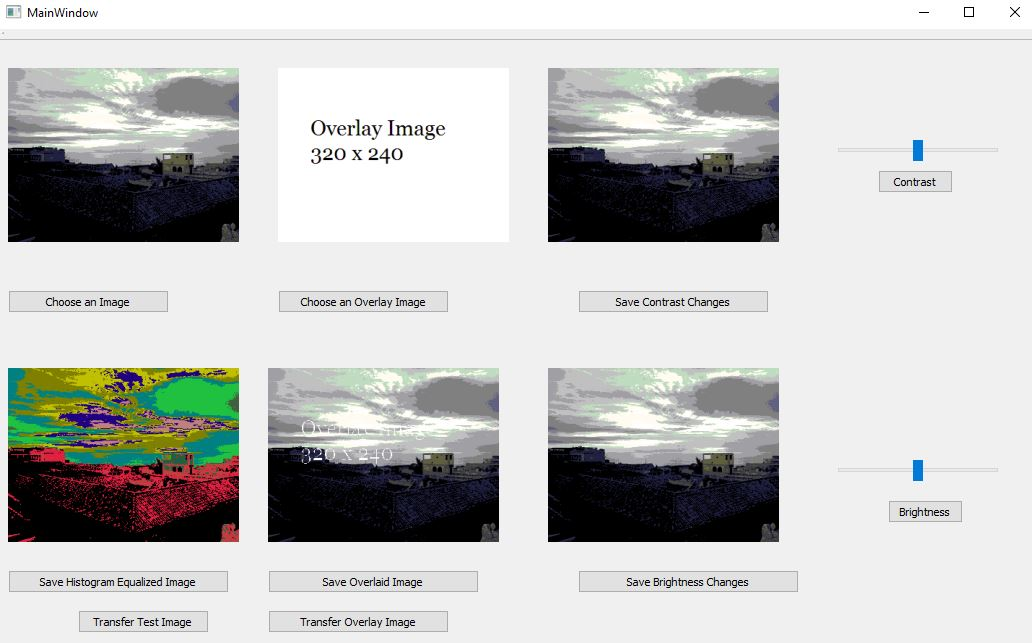
\includegraphics[width=\linewidth]{QT_GUI.jpg}
  \captionof{figure} {Layout of the GUI produced by the Qt program}
\end{Figure}

Every time new data is sent from the QT program (GUI), it is appended with 1 character that is used to determine what type of data we are receiving:

\begin{itemize}
  \item 0 : original image
  \item 1 : brightness slider
  \item 2 : contrast slider
  \item 3 : overlay image
\end{itemize}


{\bf-Sending Original Image:}
The first button, Transfer Test Image, when pressed will first send the value of 0 to signify the transfer of the original image is about to begin. Second, the pixels of the original image are sent to the FPGA through the RS232 port. The function, on\_transferTest\_clicked(), iterates through the original image pixel vector and sends each pixel value for the entire 320x240 original image bitmap.
The second button, Transfer Overlay Image, when pressed will first send the value of 3 to signify the transfer of the overlay image is about to begin. Second, the pixels of the overlay image are sent to the FPGA through the RS232 port. The function, on\_transferOverlay\_clicked(), iterates through the overlay image pixels and sends each pixel for the entire 320x240 overlay image bitmap.

{\bf-Sending Overlay Image:}
The brightness slider function, on\_brightnessSlider\_valueChanged(int value), was updated to first send a value of 1 to signify the transfer of the brightness slider value is about to begin. Second, the value of the slider, when changed, is sent to the FPGA.
The contrast slider function, on\_contrastSlider\_valueChanged(int value), was updated to first send a value of 2 to signify the transfer of the brightness slider value is about to begin. Second, the value of the slider, when changed, is sent to the FPGA.\\

{\bf-Sending Brightness Slider Value :}
The brightness slider function, on\_brightnessSlider\_valueChanged(int value), was updated to first send a value of 1 to signify the transfer of the brightness slider value is about to begin. Second, the value of the slider, when changed, is sent to the FPGA.

{\bf-Sending Contrast Slider Value :}
The contrast slider function, on\_contrastSlider\_valueChanged(int value), was updated to first send a value of 2 to signify the transfer of the brightness slider value is about to begin. Second, the value of the slider, when changed, is sent to the FPGA.\\

{\bf DE2-115 and Nios II functionality}\\
The majority of the functionality on the FPGA side is provided by the C program that is loaded to the NIOS II processor (Media Computer).\\

{\bf-Receiving data:}
The C program remains idle continuously going through an infinite while loop, awaiting data to be received from the Qt program.
Every time new data is sent from the QT program (GUI), it is appended with 1 character that is used to determine what type of data we are receiving, which was mentioned in a previous section.


{\bf-Receiving original image:}
When the FPGA receives an original image through the RS232 connection, the flow of execution enters 2 nested for loops that access each individual element of the pixel buffer, row by row starting from the top left of the image (0,0). The way an image is sent from QT is done pixel by pixel. Therefore, the C program waits for a new value to be received by reading RVALID and checking if it is 1.The received pixel value (which is an int from 0 to 31) is then used to give a new value to the variable pix in such a way that all RGB values have the received pixel value.  
This is done with this line of code : \\
pix = (data sla 11) + (data  sla 6) + data;\\

\begin{Figure}
 \centering
 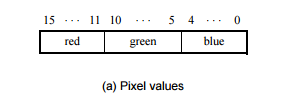
\includegraphics[width=\linewidth]{pix.png}
  \captionof{figure} {RGB layout in pixel buffer.}
\end{Figure}


{\bf-Receiving overlay image:}
When receiving an overlay image, the process of loading the individual pixels and writing them to the pixel buffer differs from the routine followed for the original image. The C program enters a loop in which it awaits data by checking RVALID, and when a character is received it is stored in an array named OverlayImage[]. Once all the pixels have been received, the entire pixel buffer is traversed while checking the corresponding values of the overlay image. If the value in the OverlayImage[] array is less than 17 ( the overlay image was created in paint, therefore the text is black but the border of the characters is actually grey) then the value from the array is writen to the pixel buffer, overwriting the pixel of the original image. Otherwise the original pixel remains unchanged.\\

{\bf-Receiving a brightness slider value:}

Upon receiving a slider value from Qt a new variable “change” is calculated using the following line of code:
int change = (brightness - prevSlider) * 1/5 ;
Where brightness is the  value of the slider and prevSlider is the last value the slider had (initially it is set to 50).
Before applying the changes, it is ensured that the new value of the pixel does not exceed the range of 0-31.
This change is then added to the pixels(in the pixel buffer) of the original image thus adjusting the brightness of the image.\\

{\bf-Receiving a contrast slider value:}
-Receiving a contrast slider value:
Similarly to the brightness slider, when the contrast value is received, the value is processed based on the code in the Appendix and the value of the original image is adjusted accordingly.










%----------------------------------------------------------------------------------------
%		EVALUATION
%----------------------------------------------------------------------------------------
\begin{center}
\large{III. Evaluation(Megan Rowland)}
\end{center}

When running the QT GUI, a user will have the option to select an original image (this was implemented in Milestone 2: Creating a Graphical User Interface (GUI) for processing images). When the button, Transfer Test Image, is pressed the original image will be transferred from QT through the RS232 port to the FPGA and display via the VGA port to an external monitor through the pixel buffer on the DE2-115 Media Computer. 

\begin{Figure}
 \centering
 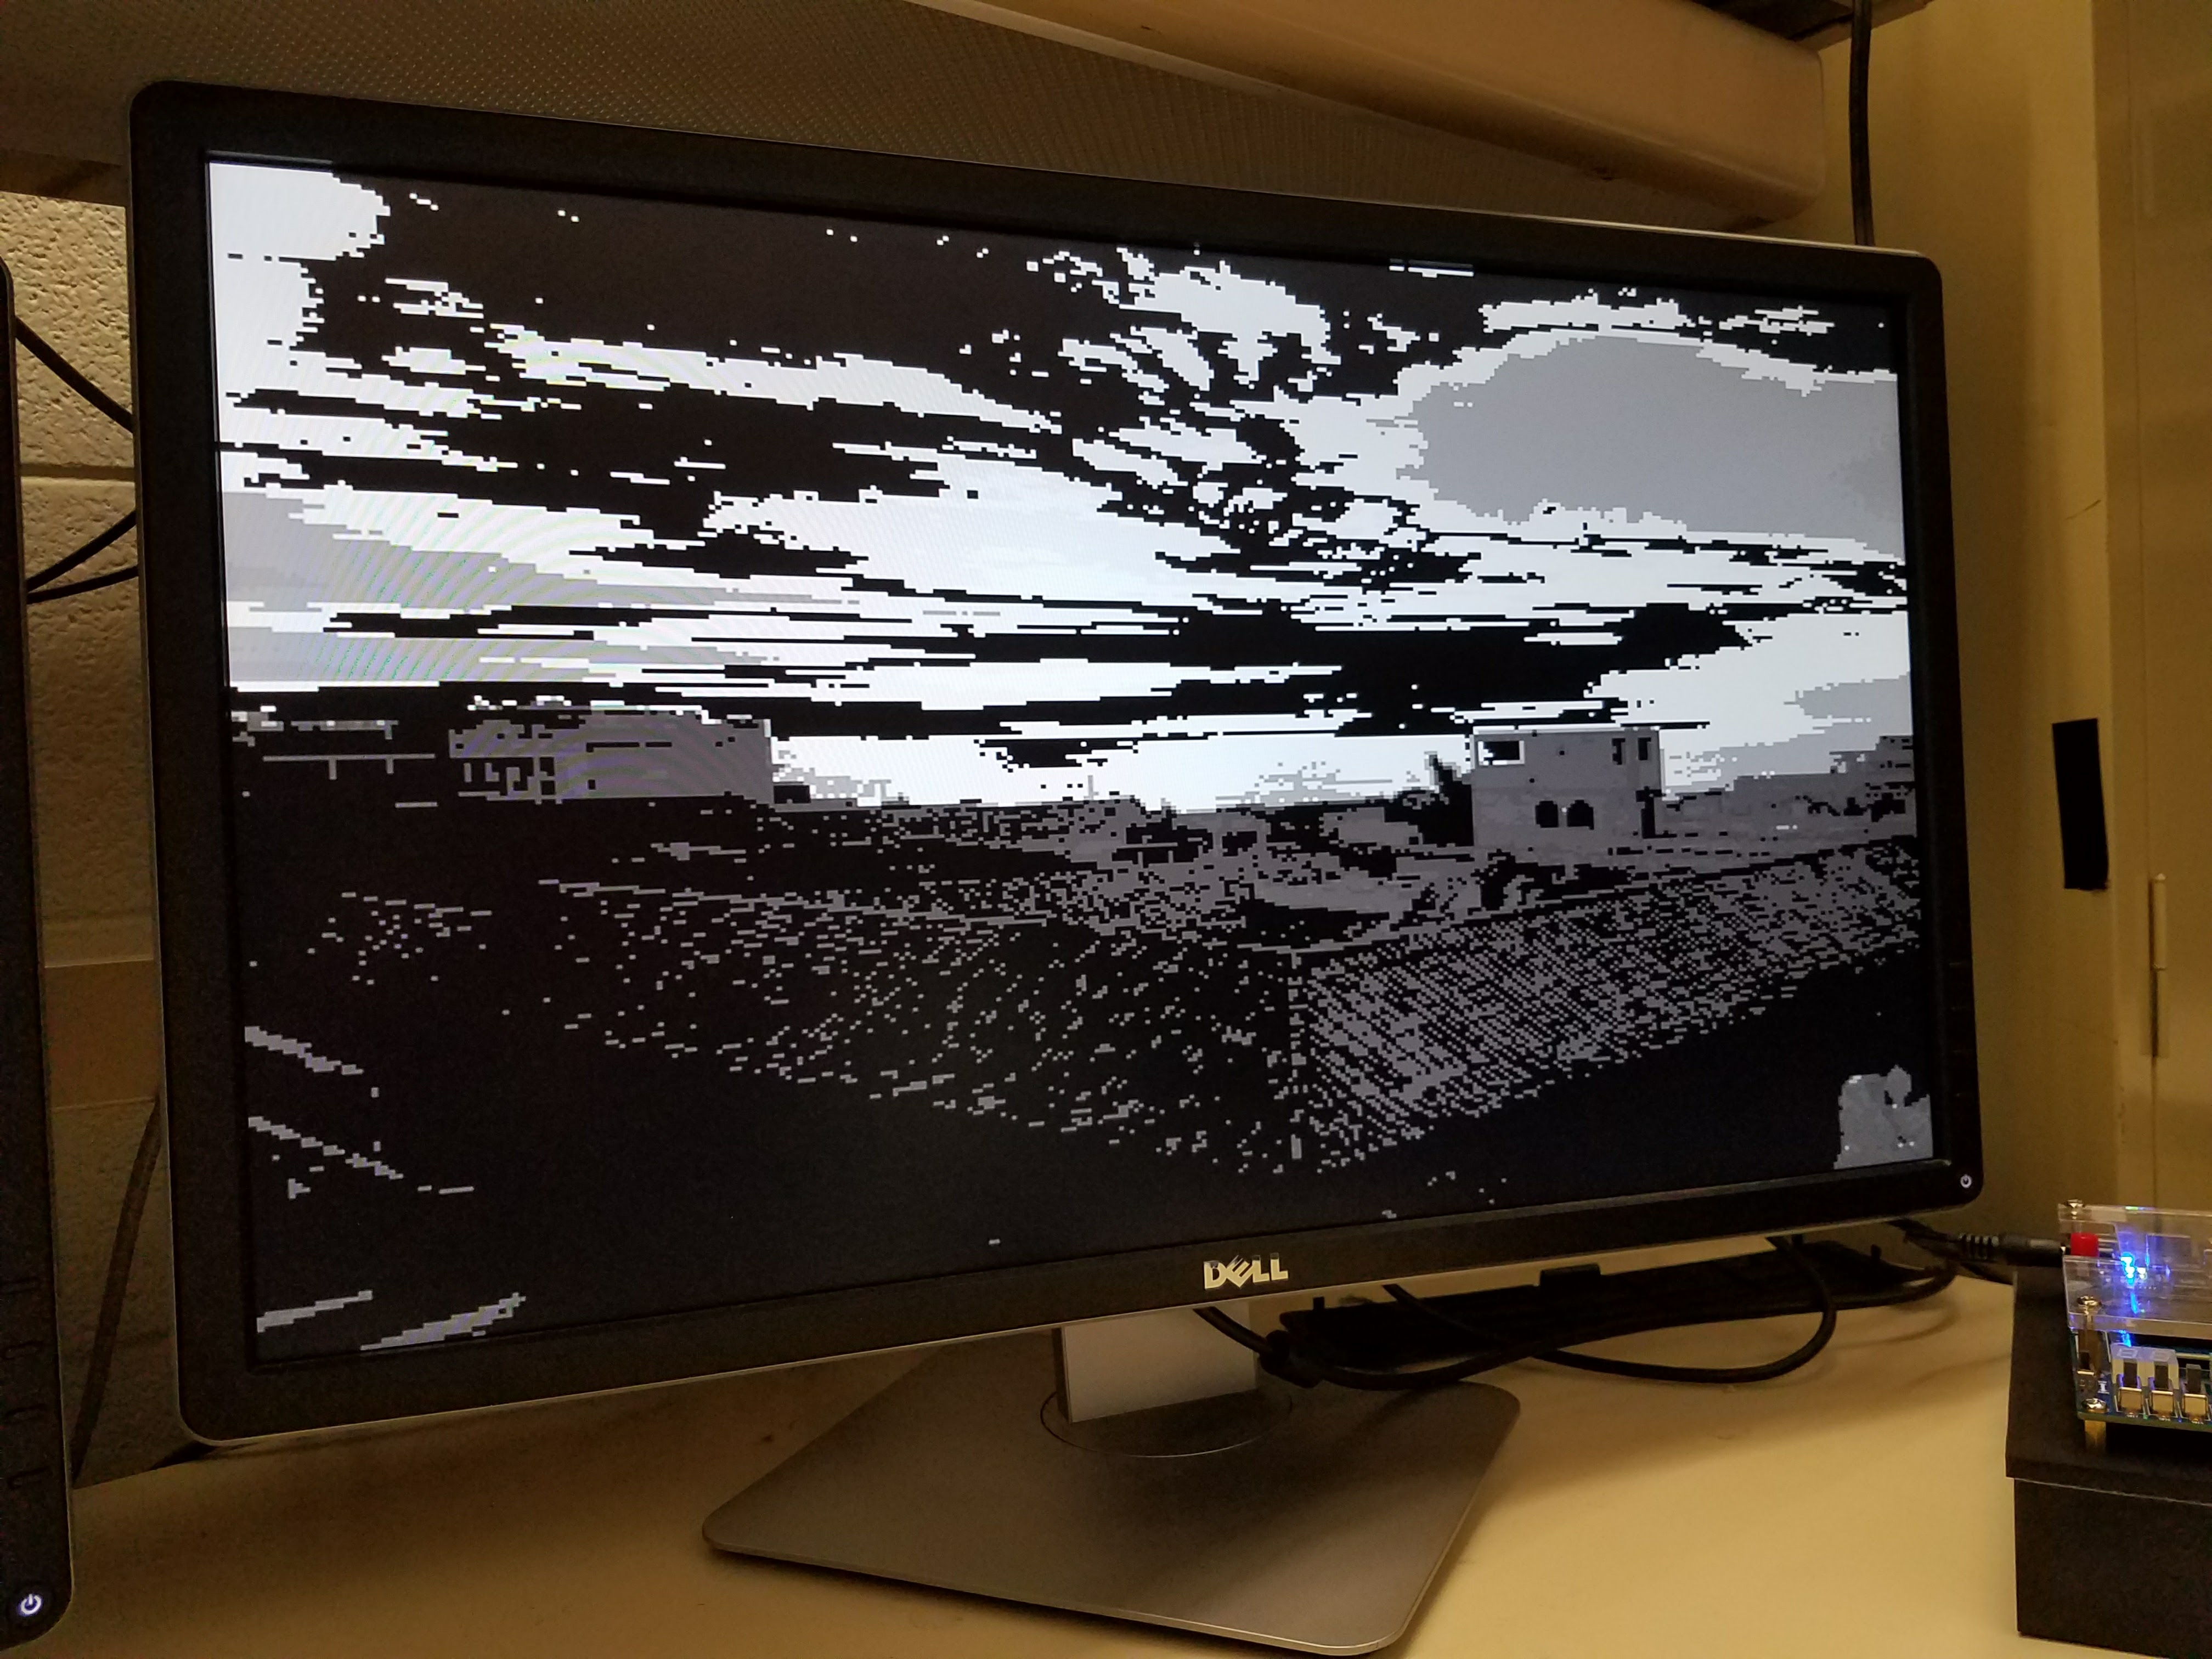
\includegraphics[width=\linewidth]{original_image_transfer.jpg}
  \captionof{figure} {Display of "test2.bmp" scaled to 320x240 generated by the VGA}
\end{Figure}


%<<original_image_transfer.jpg>>
When running the QT GUI, a user will also have the option to select an overlay image (this was also implemented in Milestone 2: Creating a Graphical User Interface (GUI) for processing images). When the button, Transfer Overlay Image, is pressed the overlay image will be transferred from QT through the RS232 port and stored in memory on the FPGA. The C program will iterate through the stored values for the pixels of the overlay image and any pixel on the overlay image that is black will be overwritten in the pixel buffer as the value for white. When this is complete the overlaid image will be displayed via the VGA port to an external monitor.

\begin{Figure}
 \centering
 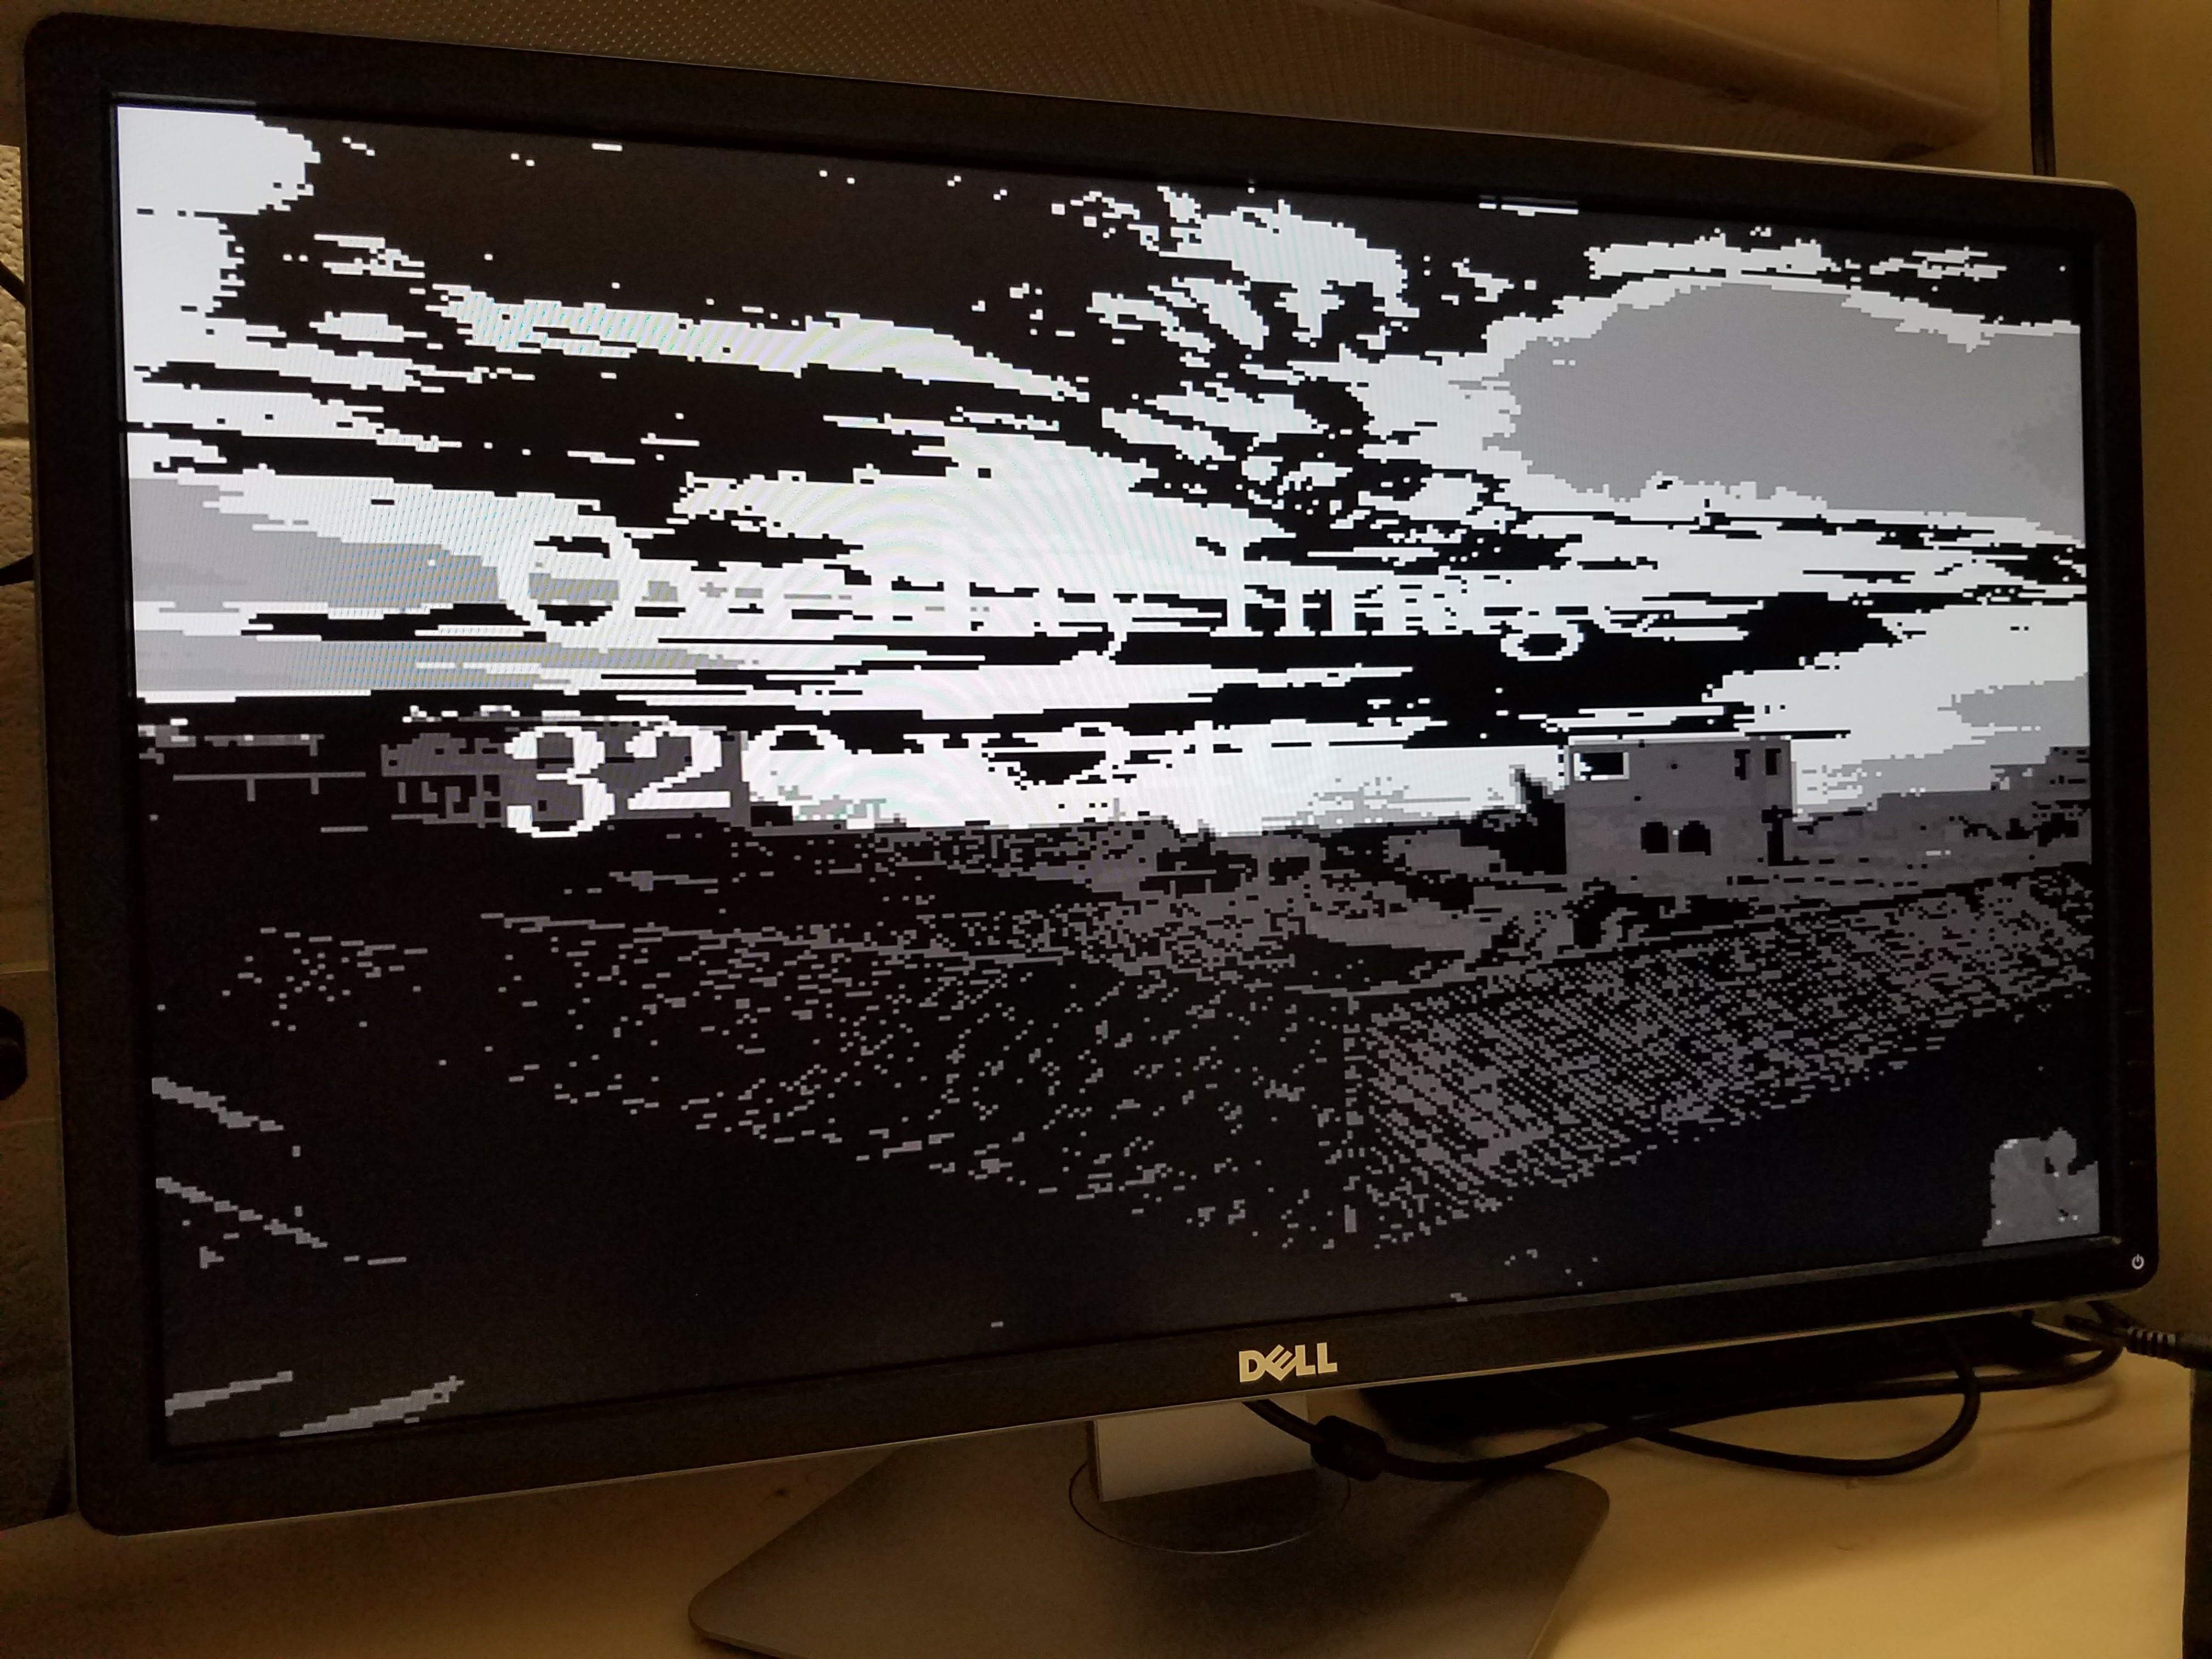
\includegraphics[width=\linewidth]{overlaid_image.jpg}
  \captionof{figure} {Display of "test2.bmp" overlaid with image displaying "Overlay Image" in text}
\end{Figure}

%<<overlaid_image.jpg>>

When the brightness slider is moved to the left or right, the new value of the slider is sent from QT through the RS232 port. This value is then used on the FPGA to increase or decrease the brightness of the image displayed on the external monitor. 
When the contrast slider is moved to the left or right, the new value of the slider is sent from QT through the RS232 port. This value is then used on the FPGA to increase or decrease the contrast of the image displayed on the external monitor.


%----------------------------------------------------------------------------------------
%		DISCUSSION
%----------------------------------------------------------------------------------------
\begin{center}
\large{IV. Discussion(Michael Micros)}
\end{center}
From the results displayed in the evaluation,  much more could be done to improve the performance of our design. Improvements can be made as to the quality of brightness and contrast adjustment performed on the original image. Unfortunately, the speed at which images are loaded or updated is limited to the processing power of the FPGA, which is out of our control. Another limitation imposed by the FPGA is the resolution of the displayed images via VGA, which is limited to 320x240. Finally, an improvement that could be made is to add black or gray pixels to the border of the white overlaid text so as to ensure the visiblility of the overlay image over whte background.


%----------------------------------------------------------------------------------------
%		REFERENCES
%----------------------------------------------------------------------------------------
\begin{center}
\large{IV. References}
\end{center}

[1]	H. Edwards et al., “Image Processing: Overlaying and Histogram Equalization,” Old Dominion University, Norfolk, Virginia, Feb 2017.

[2]     M. Micros et al., “ Creating Graphical User Interface GUI for processing images,” Old Dominion University, Norfolk, Virginia, Feb 2017.

[3]	J. Rigney et al., “Implementing AND gates, 8-bit binary counters and 2-Digit BCD counters using DE2-115 FPGA,” Old Dominion University, Norfolk, Virginia,  Mar 2017.

[4]	M. Rowland et al.,  Establishing communication between Qt program and DE2-115 FPGA,” Old Dominion University, Norfolk, Virginia, Apr 2017.


\end{multicols*}


%----------------------------------------------------------------------------------------
%		APPENDIX
%----------------------------------------------------------------------------------------
\begin{center}
\large{IV. Appendix}
\end{center}


\begin{Figure}
 \centering
 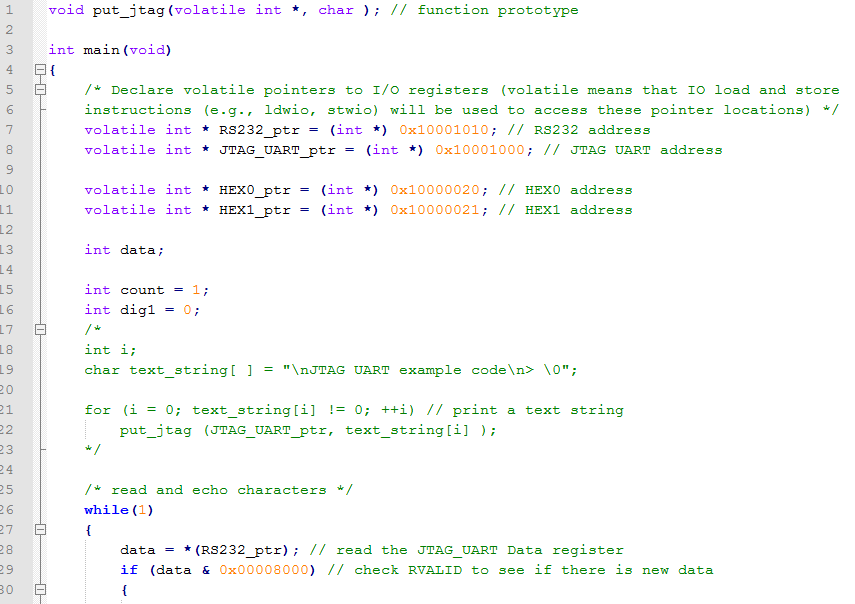
\includegraphics[width=\linewidth]{c1.png}
\end{Figure}

\begin{Figure}
 \centering
 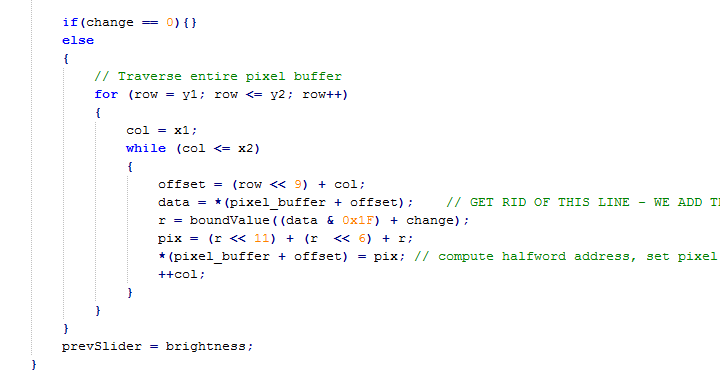
\includegraphics[width=\linewidth]{c2.png}
\end{Figure}


\begin{Figure}
 \centering
 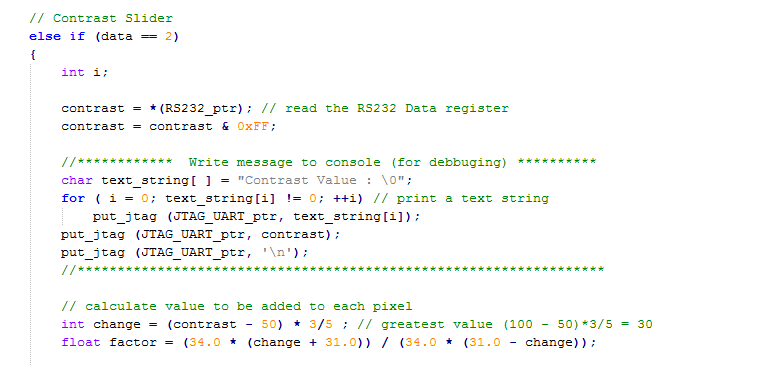
\includegraphics[width=\linewidth]{c3.png}
\end{Figure}

\begin{Figure}
 \centering
 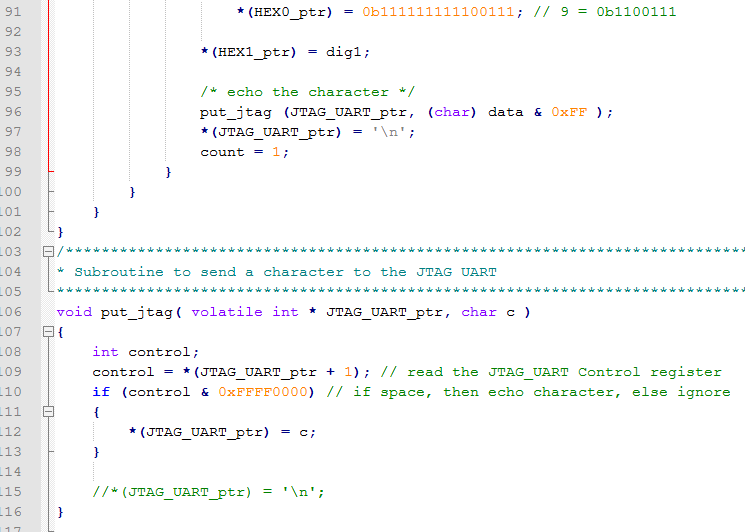
\includegraphics[width=\linewidth]{c4.png}
\end{Figure}


%----------------------------------------------------------------------------------------
\end{document}
